\documentclass[crop,tikz]{standalone}
\usetikzlibrary{backgrounds}
\colorlet{blue}{cyan}
\tikzset{
  inverted/.style = {
    every path/.style = {draw=white,text=white},
    background rectangle/.style={fill},
    show background rectangle
  }
}

\tikzset{>=latex}
\usetikzlibrary{decorations.markings}
\colorlet{green}{green}

\begin{document}
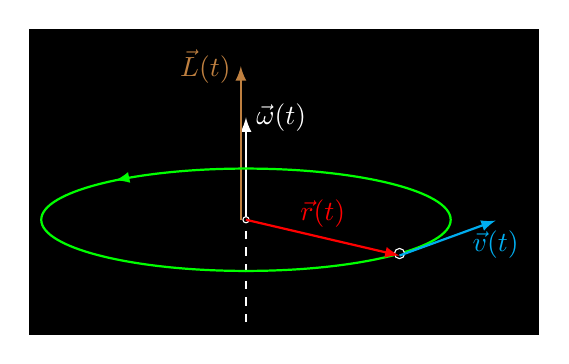
\begin{tikzpicture}[inverted,scale=1.3]
  \draw[dashed,thick] (0,1) -- (0,2);
  \draw[->,thick] (0,2) -- +(0,1) node[right] {$\vec{\omega}(t)$};
  \draw[->,brown,thick] (-0.05,2) -- +(0,1.5) node[left] {$\vec{L}(t)$};
  \fill (0,2) circle (0.03);
  \draw[thick,
        decoration={markings, mark=at position 0.4 with {\arrow{>}}},
        postaction={decorate},
        green
  ] (0,2) ellipse (2 and 0.5);
  \fill (1.5,1.67) circle (0.05);
  \draw[->,red ,thick] (0,2) -- node[above] {$\vec{r}(t)$} (1.5,1.65);
  \draw[->,blue,thick] (1.5,1.65) -- +(20:1) node[below] {$\vec{v}(t)$};
\end{tikzpicture}
\end{document}
